\documentclass[12pt]{beamer}\usepackage[]{graphicx}\usepackage[]{color}
%% maxwidth is the original width if it is less than linewidth
%% otherwise use linewidth (to make sure the graphics do not exceed the margin)
\makeatletter
\def\maxwidth{ %
  \ifdim\Gin@nat@width>\linewidth
    \linewidth
  \else
    \Gin@nat@width
  \fi
}
\makeatother

\definecolor{fgcolor}{rgb}{0.345, 0.345, 0.345}
\newcommand{\hlnum}[1]{\textcolor[rgb]{0.686,0.059,0.569}{#1}}%
\newcommand{\hlstr}[1]{\textcolor[rgb]{0.192,0.494,0.8}{#1}}%
\newcommand{\hlcom}[1]{\textcolor[rgb]{0.678,0.584,0.686}{\textit{#1}}}%
\newcommand{\hlopt}[1]{\textcolor[rgb]{0,0,0}{#1}}%
\newcommand{\hlstd}[1]{\textcolor[rgb]{0.345,0.345,0.345}{#1}}%
\newcommand{\hlkwa}[1]{\textcolor[rgb]{0.161,0.373,0.58}{\textbf{#1}}}%
\newcommand{\hlkwb}[1]{\textcolor[rgb]{0.69,0.353,0.396}{#1}}%
\newcommand{\hlkwc}[1]{\textcolor[rgb]{0.333,0.667,0.333}{#1}}%
\newcommand{\hlkwd}[1]{\textcolor[rgb]{0.737,0.353,0.396}{\textbf{#1}}}%

\usepackage{framed}
\makeatletter
\newenvironment{kframe}{%
 \def\at@end@of@kframe{}%
 \ifinner\ifhmode%
  \def\at@end@of@kframe{\end{minipage}}%
  \begin{minipage}{\columnwidth}%
 \fi\fi%
 \def\FrameCommand##1{\hskip\@totalleftmargin \hskip-\fboxsep
 \colorbox{shadecolor}{##1}\hskip-\fboxsep
     % There is no \\@totalrightmargin, so:
     \hskip-\linewidth \hskip-\@totalleftmargin \hskip\columnwidth}%
 \MakeFramed {\advance\hsize-\width
   \@totalleftmargin\z@ \linewidth\hsize
   \@setminipage}}%
 {\par\unskip\endMakeFramed%
 \at@end@of@kframe}
\makeatother

\definecolor{shadecolor}{rgb}{.97, .97, .97}
\definecolor{messagecolor}{rgb}{0, 0, 0}
\definecolor{warningcolor}{rgb}{1, 0, 1}
\definecolor{errorcolor}{rgb}{1, 0, 0}
\newenvironment{knitrout}{}{} % an empty environment to be redefined in TeX

\usepackage{alltt}
\usepackage{graphicx}
\usepackage{tikz}
\setbeameroption{hide notes}
\setbeamertemplate{note page}[plain]
\usepackage{listings}

% get rid of junk
\usetheme{default}
\usefonttheme[onlymath]{serif}
\beamertemplatenavigationsymbolsempty
\hypersetup{pdfpagemode=UseNone} % don't show bookmarks on initial view

% named colors
\definecolor{offwhite}{RGB}{255,250,240}
\definecolor{gray}{RGB}{155,155,155}

\ifx\notescolors\undefined % slides

  \definecolor{foreground}{RGB}{80,80,80}
  \definecolor{background}{RGB}{255,255,255}
  \definecolor{title}{RGB}{255,199,0}
  \definecolor{subtitle}{RGB}{89,132,212}
  \definecolor{hilit}{RGB}{248,117,79}
  \definecolor{vhilit}{RGB}{255,111,207}
  \definecolor{lolit}{RGB}{200,200,200}
  \definecolor{lit}{RGB}{255,199,0}
  \definecolor{mdlit}{RGB}{89,132,212}
  \definecolor{link}{RGB}{248,117,79}

\else % notes
  \definecolor{background}{RGB}{255,255,255}
  \definecolor{foreground}{RGB}{24,24,24}
  \definecolor{title}{RGB}{27,94,134}
  \definecolor{subtitle}{RGB}{22,175,124}
  \definecolor{hilit}{RGB}{122,0,128}
  \definecolor{vhilit}{RGB}{255,0,128}
  \definecolor{lolit}{RGB}{95,95,95}
\fi
\definecolor{nhilit}{RGB}{128,0,128}  % hilit color in notes
\definecolor{nvhilit}{RGB}{255,0,128} % vhilit for notes

\newcommand{\hilit}{\color{hilit}}
\newcommand{\vhilit}{\color{vhilit}}
\newcommand{\nhilit}{\color{nhilit}}
\newcommand{\nvhilit}{\color{nvhilit}}
\newcommand{\lit}{\color{lit}}
\newcommand{\mdlit}{\color{mdlit}}
\newcommand{\lolit}{\color{lolit}}

% use those colors
\setbeamercolor{titlelike}{fg=title}
\setbeamercolor{subtitle}{fg=subtitle}
\setbeamercolor{frametitle}{fg=gray}
\setbeamercolor{structure}{fg=subtitle}
\setbeamercolor{institute}{fg=lolit}
\setbeamercolor{normal text}{fg=foreground,bg=background}
%\setbeamercolor{item}{fg=foreground} % color of bullets
%\setbeamercolor{subitem}{fg=hilit}
%\setbeamercolor{itemize/enumerate subbody}{fg=lolit}
\setbeamertemplate{itemize subitem}{{\textendash}}
\setbeamerfont{itemize/enumerate subbody}{size=\footnotesize}
\setbeamerfont{itemize/enumerate subitem}{size=\footnotesize}

% center title of slides
\setbeamertemplate{blocks}[rounded]
\setbeamertemplate{frametitle}[default][center]
% margins
\setbeamersize{text margin left=25pt,text margin right=25pt}

% page number
\setbeamertemplate{footline}{%
    \raisebox{5pt}{\makebox[\paperwidth]{\hfill\makebox[20pt]{\lolit
          \scriptsize\insertframenumber}}}\hspace*{5pt}}

% add a bit of space at the top of the notes page
\addtobeamertemplate{note page}{\setlength{\parskip}{12pt}}

% default link color
\hypersetup{colorlinks, urlcolor={link}}

\ifx\notescolors\undefined % slides
  % set up listing environment
  \lstset{language=bash,
          basicstyle=\ttfamily\scriptsize,
          frame=single,
          commentstyle=,
          backgroundcolor=\color{darkgray},
          showspaces=false,
          showstringspaces=false
          }
\else % notes
  \lstset{language=bash,
          basicstyle=\ttfamily\scriptsize,
          frame=single,
          commentstyle=,
          backgroundcolor=\color{offwhite},
          showspaces=false,
          showstringspaces=false
          }
\fi

% a few macros
\newcommand{\code}[1]{\texttt{#1}}
\newcommand{\hicode}[1]{{\hilit \texttt{#1}}}
\newcommand{\bb}[1]{\begin{block}{#1}}
\newcommand{\eb}{\end{block}}
\newcommand{\bi}{\begin{itemize}}
%\newcommand{\bbi}{\vspace{24pt} \begin{itemize} \itemsep8pt}
\newcommand{\bbi}{\vspace{4pt} \begin{itemize} \itemsep8pt}
\newcommand{\ei}{\end{itemize}}
\newcommand{\bv}{\begin{verbatim}}
\newcommand{\ev}{\end{verbatim}}
\newcommand{\ig}{\includegraphics}
\newcommand{\subt}[1]{{\footnotesize \color{subtitle} {#1}}}
\newcommand{\ttsm}{\tt \small}
\newcommand{\ttfn}{\tt \footnotesize}
\newcommand{\figh}[2]{\centerline{\includegraphics[height=#2\textheight]{#1}}}
\newcommand{\figw}[2]{\centerline{\includegraphics[width=#2\textwidth]{#1}}}



%------------------------------------------------
% end of header
%------------------------------------------------

\title{Graphics Devices}
\subtitle{Stat 133}
\author{\href{http://www.gastonsanchez.com}{Gaston Sanchez}}
\institute{Department of Statistics, UC{\textendash}Berkeley}
\date{\href{http://www.gastonsanchez.com}{\tt \scriptsize \color{foreground} gastonsanchez.com}
\\[-4pt]
\href{http://github.com/gastonstat}{\tt \scriptsize \color{foreground} github.com/gastonstat}
\\[-4pt]
{\scriptsize Course web: \href{http://www.gastonsanchez.com/teaching/stat133}{\tt gastonsanchez.com/teaching/stat133}}
}
\IfFileExists{upquote.sty}{\usepackage{upquote}}{}
\begin{document}


{
  \setbeamertemplate{footline}{} % no page number here
  \frame{
    \titlepage
  } 
}

%------------------------------------------------

\begin{frame}
\frametitle{Graphics Formats}

{\Large How to produce graphical output in different formats}

\end{frame}

%------------------------------------------------

\begin{frame}
\frametitle{Plotting options}

\centerline{\Large \mdlit When creating a plot in R ...}

\vspace{18pt}

\centerline{\Large Screen display \quad OR \quad Save in File}

\end{frame}

%------------------------------------------------

\begin{frame}[fragile]
\frametitle{Plotting options}

\begin{knitrout}\footnotesize
\definecolor{shadecolor}{rgb}{0.969, 0.969, 0.969}\color{fgcolor}

{\centering 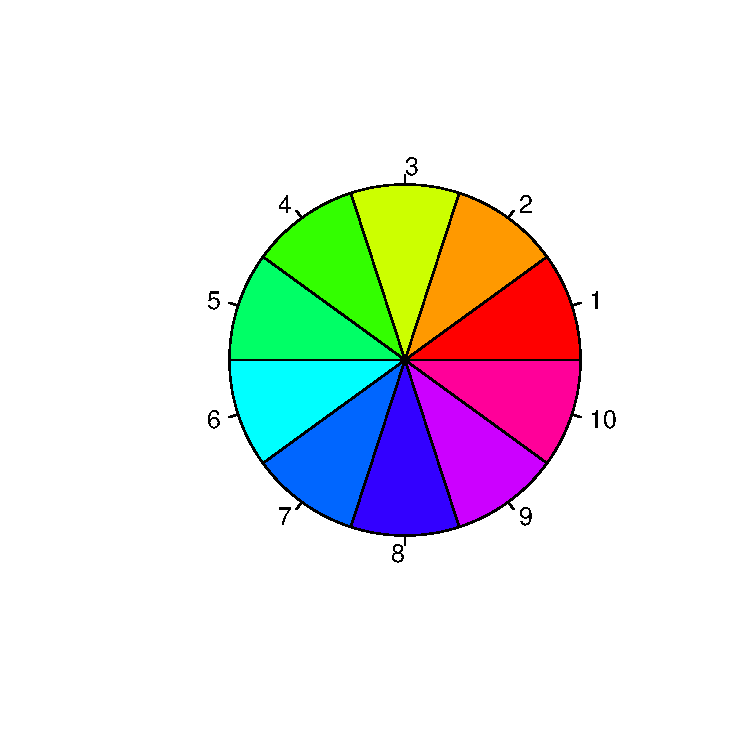
\includegraphics[width=.8\linewidth,height=.8\linewidth]{figure/unnamed-chunk-1-1} 

}



\end{knitrout}

\end{frame}

%------------------------------------------------

\begin{frame}[fragile]
\frametitle{Plotting options}

\begin{knitrout}\footnotesize
\definecolor{shadecolor}{rgb}{0.969, 0.969, 0.969}\color{fgcolor}\begin{kframe}
\begin{alltt}
\hlcom{# displaying on screen}
\hlkwd{pie}\hlstd{(}\hlkwd{rep}\hlstd{(}\hlnum{1}\hlstd{,} \hlnum{10}\hlstd{),} \hlkwc{col} \hlstd{=} \hlkwd{rainbow}\hlstd{(}\hlnum{10}\hlstd{))}


\hlcom{# saving to a file}
\hlkwd{pdf}\hlstd{(}\hlstr{"dummy_plot.pdf"}\hlstd{)}
\hlkwd{pie}\hlstd{(}\hlkwd{rep}\hlstd{(}\hlnum{1}\hlstd{,} \hlnum{10}\hlstd{),} \hlkwc{col} \hlstd{=} \hlkwd{rainbow}\hlstd{(}\hlnum{10}\hlstd{))}
\hlkwd{dev.off}\hlstd{()}
\end{alltt}
\end{kframe}
\end{knitrout}

\end{frame}

%------------------------------------------------

\begin{frame}
\frametitle{Plots with R}

\bb{What happens whe you make a plot in R?}
\bbi
  \item Graphical output is directed to a \textbf{graphics device}
  \item A graphics device must be opened
  \item Subsequent calls to graphics functions directed to a device
  \item Finally, the graphics device is closed
\ei
\eb

\end{frame}

%------------------------------------------------

\begin{frame}
\frametitle{Graphics Devices}

\bb{2 types of graphics devices}
\bbi
  \item \textbf{Screen} devices
  \item \textbf{File} devices
  \item For more info see \code{?Devices}
\ei
\eb

\end{frame}

%------------------------------------------------

\begin{frame}
\frametitle{Graphics Devices}

\bb{Default plotting}
\bi
  \item The default plotting is made via a screen device
  \item e.g. when you call \code{plot()}, \code{pie()}, or \code{barplot()}
  \item The plot appears on a given screen device
  \item If you use RStudio, the plot appears of the RStudio graphics device
  \item You can specify a particular screen device
\ei
\eb

\end{frame}

%------------------------------------------------

\begin{frame}
\frametitle{Screen Devices}

\begin{center}
  \begin{tabular}{l l}
  \multicolumn{2}{c}{\textbf{Screen Devices functions}} \\
  \hline
  Function & Graphical Format \\
    \hline
    \code{x11()} & \textit{X Window} window (Cairo graphics) \\
     & \\
    \code{windows()} & \textit{Microsoft Windows} window \\
     & \\
    \code{quartz()} & \textit{MacOS X Quartz} window \\
    \hline
 \end{tabular}
\end{center}

When displaying on screen, we usually don't have to worry about graphics devices
\end{frame}

%------------------------------------------------

\begin{frame}[fragile]
\frametitle{Quick examples}

If you have a mac try this:
\begin{knitrout}\footnotesize
\definecolor{shadecolor}{rgb}{0.969, 0.969, 0.969}\color{fgcolor}\begin{kframe}
\begin{alltt}
\hlkwd{quartz}\hlstd{()}   \hlcom{# open screen device}
\hlkwd{plot}\hlstd{(}\hlnum{1}\hlopt{:}\hlnum{10}\hlstd{,} \hlnum{1}\hlopt{:}\hlnum{10}\hlstd{,} \hlkwc{pch} \hlstd{=} \hlnum{19}\hlstd{)}  \hlcom{# plot something}
\end{alltt}
\end{kframe}
\end{knitrout}

\bigskip
After inspecting the plot ...
\begin{knitrout}\footnotesize
\definecolor{shadecolor}{rgb}{0.969, 0.969, 0.969}\color{fgcolor}\begin{kframe}
\begin{alltt}
\hlcom{# close device}
\hlkwd{dev.off}\hlstd{()}
\end{alltt}
\end{kframe}
\end{knitrout}

\end{frame}

%------------------------------------------------

\begin{frame}[fragile]
\frametitle{Quick examples}

If you have a PC try this:
\begin{knitrout}\footnotesize
\definecolor{shadecolor}{rgb}{0.969, 0.969, 0.969}\color{fgcolor}\begin{kframe}
\begin{alltt}
\hlkwd{windows}\hlstd{()}  \hlcom{# open screen device}
\hlkwd{plot}\hlstd{(}\hlnum{1}\hlopt{:}\hlnum{10}\hlstd{,} \hlnum{1}\hlopt{:}\hlnum{10}\hlstd{,} \hlkwc{pch} \hlstd{=} \hlnum{19}\hlstd{)}  \hlcom{# plot something}
\end{alltt}
\end{kframe}
\end{knitrout}

\bigskip
After inspecting the plot ...
\begin{knitrout}\footnotesize
\definecolor{shadecolor}{rgb}{0.969, 0.969, 0.969}\color{fgcolor}\begin{kframe}
\begin{alltt}
\hlcom{# close device}
\hlkwd{dev.off}\hlstd{()}
\end{alltt}
\end{kframe}
\end{knitrout}

\end{frame}

%------------------------------------------------

\begin{frame}
\frametitle{Screen Devices in R}

\bbi
  \item {\hilit \code{dev.new()}} opens the default device (not in RStudio)
  \item your default device can be found with \code{options("device")}
  \item If you use RStudio to plot on screen, the device is \code{"RStudioGD"}
\ei

\end{frame}

%------------------------------------------------

\begin{frame}
\frametitle{File Devices}

\bb{File Devices}
\bbi
  \item Instead of displaying a plot on screen, we can save it to a file
  \item when saving a plot to a file you must use a \textbf{file} device
  \item each file device has its own name
  \item some devices are platform dependent
\ei
\eb

\end{frame}

%------------------------------------------------

\begin{frame}
\frametitle{File Devices}

\begin{center}
  \begin{tabular}{l l}
  \multicolumn{2}{c}{\textbf{File Devices functions}} \\
  \hline
  Function & Graphical Format \\
    \hline
    \code{postscript()} & Adobe PostScript file \\
    \code{pdf()} & Portable Document Format \\
    \code{svg()} & SVG file (Linux and MacOS X only) \\
    \code{win.metafile()} & Windows Metafile (Windows only) \\
    \code{png()} & PNG file \\
    \code{jpeg()} & JPEG file \\
    \code{bmp()} & BMP file \\
    \code{tiff()} & TIFF file \\
    \code{pictex()} & LaTeX PicTEX file \\
    \code{xfig()} & xfig FIG file \\
    \code{bitmap()} & Multiple formats via Ghostscript \\
    \hline
 \end{tabular}
\end{center}

\end{frame}

%------------------------------------------------

\begin{frame}
\frametitle{File Acronyms}

\begin{center}
  \begin{tabular}{l l}
  \multicolumn{2}{c}{\textbf{File Acronyms}} \\
  \hline
  Acronym & Description \\
    \hline
    PDF & Portable Document Format \\
    SVG & Scalable Vector Graphics \\
    PNG & Portable Network Graphics \\
    JPEG & Joint Photographic Experts Group \\
    BMP & Bitmap \\
    TIFF & Tagged Image File Format \\
    \hline
 \end{tabular}
\end{center}

\end{frame}

%------------------------------------------------

\begin{frame}
\frametitle{Output Formats}

\centerline{\Large \mdlit Graphics devices from the output format}

\bigskip

\centerline{\Large Vector \quad -vs- \quad Raster}

\end{frame}

%------------------------------------------------

\begin{frame}
\frametitle{Output Formats}

\bb{Vector Formats}
An image is described by a set of mathematical shapes (e.g. PDF, PostScript, SVG)
\eb

\bb{Raster Formats}
An image consists of an array of pixels, with information such as color recorded for each pixel (e.g. PNG, JPEG, TIFF, all screen devices)
\eb

\end{frame}

%------------------------------------------------

\begin{frame}[fragile]
\frametitle{Quick examples}

Vector format:
\begin{knitrout}\footnotesize
\definecolor{shadecolor}{rgb}{0.969, 0.969, 0.969}\color{fgcolor}\begin{kframe}
\begin{alltt}
\hlkwd{pdf}\hlstd{(}\hlstr{"dummy_plot.pdf"}\hlstd{)}  \hlcom{# open device}
\hlkwd{pie}\hlstd{(}\hlkwd{rep}\hlstd{(}\hlnum{1}\hlstd{,} \hlnum{10}\hlstd{),} \hlkwc{col} \hlstd{=} \hlkwd{rainbow}\hlstd{(}\hlnum{10}\hlstd{))}  \hlcom{# plot something}
\hlkwd{dev.off}\hlstd{()}  \hlcom{# close device}
\end{alltt}
\end{kframe}
\end{knitrout}

\bigskip

Raster format:
\begin{knitrout}\footnotesize
\definecolor{shadecolor}{rgb}{0.969, 0.969, 0.969}\color{fgcolor}\begin{kframe}
\begin{alltt}
\hlkwd{png}\hlstd{(}\hlstr{"dummy_plot.png"}\hlstd{)}  \hlcom{# open device}
\hlkwd{pie}\hlstd{(}\hlkwd{rep}\hlstd{(}\hlnum{1}\hlstd{,} \hlnum{10}\hlstd{),} \hlkwc{col} \hlstd{=} \hlkwd{rainbow}\hlstd{(}\hlnum{10}\hlstd{))}  \hlcom{# plot something}
\hlkwd{dev.off}\hlstd{()}  \hlcom{# close device}
\end{alltt}
\end{kframe}
\end{knitrout}

\end{frame}

%------------------------------------------------

\begin{frame}
\frametitle{Vector or Raster?}

\bb{Vector Formats}
Vector formats are superior for images that need to be viewed at a variety of scales (i.e. zoom in and out).
\eb

\end{frame}

%------------------------------------------------

\begin{frame}
\frametitle{Example: vector image (pdf)}
\begin{center}
\ig[width=7cm]{images/dummy_plot.pdf}
\end{center}
\end{frame}

%------------------------------------------------

\begin{frame}
\frametitle{Vector or Raster?}

\bb{Raster Formats}
Raster formats tend to be preferred when a plot is visually complex (e.g. many data points), and it will produce smaller files if the image is very complex.
\eb

\end{frame}

%------------------------------------------------

\begin{frame}
\frametitle{Example: raster image (png)}
\begin{center}
\ig[width=7cm]{images/dummy_plot.png}
\end{center}
\end{frame}

%------------------------------------------------

\begin{frame}
\frametitle{Vector or Raster?}

If further modifications to an R plot will be made using third-party software:
\bi
  \item removing a particular form are only possibe with vector format
  \item modifying pixels of a particular color are only possible with raster formats
\ei

{\lit Keep in mind: It is easy to convert a vector format to a raster format, while the reverse is almost impossible}
\end{frame}

%------------------------------------------------

\begin{frame}
\frametitle{Vector Formats}

\bb{PDF}
\bi
  \item Good choice of static format
  \item Resizes well, usually portable
  \item Less efficient if a plot has many objects/points
  \item \code{pdf()} uses default sans-serif font (Helvetica)
  \item Other standard fonts are supported
  \item For more exotic fonts you should call \code{embedFonts()}
\ei
\eb

\end{frame}

%------------------------------------------------

\begin{frame}
\frametitle{Vector Formats}

\bb{SVG}
\bi
  \item XML-based format
  \item Good choice for web pages
  \item \code{svg()} available in Linux and Mac
  \item SVG output in Windows requires package \code{"Cairo"}
  \item Some advanced SVG features are limitted in R
\ei
\eb

\end{frame}

%------------------------------------------------

\begin{frame}
\frametitle{Vector Formats}

\bb{Windows Metafile}
\bi
  \item Vector format for Windows
  \item Plots compatible with Microsoft products (e.g. Word, Excel, PowerPoint)
  \item Can only be produced on Windows systems
\ei
\eb

\end{frame}

%------------------------------------------------

\begin{frame}
\frametitle{Raster (Bitmap) Formats}

\bb{PNG}
\bi
  \item Desirable format for simple images (most statistical graphics)
  \item Good for line drawings or images with solid colors
  \item Good for many, many objects, points=
  \item PNG uses \textbf{lossless} compression: compresses the image without losing information
  \item PNG does not resize well
  \item Consequently, PNG files can be edited without reducing quality
  \item Most web browsers can read this format natively
\ei
\eb

\end{frame}

%------------------------------------------------

\begin{frame}
\frametitle{Raster Formats}

\bb{JPEG}
\bi
  \item Good for photographs or natural scenes
  \item JPEG uses \textbf{lossy} compression: compresses the image with some information loss
  \item Consequently, repeatedly editing a JPEG filewill result in quality reduction
  \item JPEG does not resize well
  \item Better suited for complex images with lots of different regions (like photographs)
\ei
\eb

\end{frame}

%------------------------------------------------

\begin{frame}
\frametitle{Raster Formats}

\bb{TIFF}
\bi
  \item Sophisticated format that allows multiple pages of raster output within a single file
  \item Supports lossless compression
  \item Less supported by web browsers
  \item Preferred format for publishers of books or journal articles
\ei
\eb

\end{frame}

%------------------------------------------------

\begin{frame}
\frametitle{Raster Formats}

\bb{Image Size}
\bi
  \item Size of Raster images is specified in number of pixels (rahter than physical size in inches)
  \item The physical size of a raster image is determined by the \textbf{resolution} at which it is viewed
  \item e.g. PNG image 72 pixels wide will be 1 inch wide when viewed on a screen with a resolution of 72 dpi (dots per inch)
  \item e.g. PNG image 72 pixels wide will be 0.75 inches wide on a screen with a resolution of 96 dpi
\ei
\eb

\end{frame}

%------------------------------------------------

\begin{frame}
\frametitle{Extension Packages}

\begin{center}
  \begin{tabular}{l l l}
  \multicolumn{3}{c}{\textbf{Extension functions and packages}} \\
  \hline
  Function & Format & Package \\
    \hline
    \code{Cairo()} & Multiple formats & \code{"Cairo"} \\
    \code{tikz()} & LaTeX PGF, TikZ file & \code{"tikzDevice"} \\
    \code{devSVGTips()} & SVG file & \code{"RSVGTipsDevice"} \\
    \code{JavaGD} & Java Swing window & \code{"JavaGD"} \\
    \hline
 \end{tabular}
\end{center}

\end{frame}

%------------------------------------------------

\begin{frame}[fragile]
\frametitle{Data \code{mtcars}}

\begin{knitrout}\tiny
\definecolor{shadecolor}{rgb}{0.969, 0.969, 0.969}\color{fgcolor}\begin{kframe}
\begin{alltt}
\hlkwd{head}\hlstd{(mtcars,} \hlkwc{n} \hlstd{=} \hlnum{10}\hlstd{)}
\end{alltt}
\begin{verbatim}
##                    mpg cyl  disp  hp drat    wt  qsec vs am gear carb
## Mazda RX4         21.0   6 160.0 110 3.90 2.620 16.46  0  1    4    4
## Mazda RX4 Wag     21.0   6 160.0 110 3.90 2.875 17.02  0  1    4    4
## Datsun 710        22.8   4 108.0  93 3.85 2.320 18.61  1  1    4    1
## Hornet 4 Drive    21.4   6 258.0 110 3.08 3.215 19.44  1  0    3    1
## Hornet Sportabout 18.7   8 360.0 175 3.15 3.440 17.02  0  0    3    2
## Valiant           18.1   6 225.0 105 2.76 3.460 20.22  1  0    3    1
## Duster 360        14.3   8 360.0 245 3.21 3.570 15.84  0  0    3    4
## Merc 240D         24.4   4 146.7  62 3.69 3.190 20.00  1  0    4    2
## Merc 230          22.8   4 140.8  95 3.92 3.150 22.90  1  0    4    2
## Merc 280          19.2   6 167.6 123 3.92 3.440 18.30  1  0    4    4
\end{verbatim}
\end{kframe}
\end{knitrout}

\end{frame}

%------------------------------------------------

\begin{frame}[fragile]
\frametitle{Different sizes - same resolution}

\begin{knitrout}\footnotesize
\definecolor{shadecolor}{rgb}{0.969, 0.969, 0.969}\color{fgcolor}\begin{kframe}
\begin{alltt}
\hlcom{# 600px - 500px}
\hlkwd{png}\hlstd{(}\hlkwc{file} \hlstd{=} \hlstr{"cars-600-500.png"}\hlstd{,} \hlkwc{width} \hlstd{=} \hlnum{600}\hlstd{,} \hlkwc{height} \hlstd{=} \hlnum{500}\hlstd{)}
\hlkwd{plot}\hlstd{(mtcars[ ,}\hlkwd{c}\hlstd{(}\hlstr{'hp'}\hlstd{,} \hlstr{'mpg'}\hlstd{)],} \hlkwc{type} \hlstd{=} \hlstr{"n"}\hlstd{,}
     \hlkwc{main} \hlstd{=} \hlstr{"Horsepower and Miles-per-gallon"}\hlstd{)}
\hlkwd{text}\hlstd{(mtcars[ ,}\hlkwd{c}\hlstd{(}\hlstr{'hp'}\hlstd{,} \hlstr{'mpg'}\hlstd{)],} \hlkwc{lab} \hlstd{=} \hlkwd{rownames}\hlstd{(mtcars))}
\hlkwd{dev.off}\hlstd{()}


\hlcom{# 400px - 350px}
\hlkwd{png}\hlstd{(}\hlkwc{file} \hlstd{=} \hlstr{"cars-400-350.png"}\hlstd{,} \hlkwc{width} \hlstd{=} \hlnum{400}\hlstd{,} \hlkwc{height} \hlstd{=} \hlnum{350}\hlstd{)}
\hlkwd{plot}\hlstd{(mtcars[ ,}\hlkwd{c}\hlstd{(}\hlstr{'hp'}\hlstd{,} \hlstr{'mpg'}\hlstd{)],} \hlkwc{type} \hlstd{=} \hlstr{"n"}\hlstd{,}
     \hlkwc{main} \hlstd{=} \hlstr{"Horsepower and Miles-per-gallon"}\hlstd{)}
\hlkwd{text}\hlstd{(mtcars[ ,}\hlkwd{c}\hlstd{(}\hlstr{'hp'}\hlstd{,} \hlstr{'mpg'}\hlstd{)],} \hlkwc{lab} \hlstd{=} \hlkwd{rownames}\hlstd{(mtcars))}
\hlkwd{dev.off}\hlstd{()}
\end{alltt}
\end{kframe}
\end{knitrout}

\end{frame}

%------------------------------------------------

\begin{frame}
\frametitle{cars-600-500.png -vs- cars-400-350.png}
\begin{center}
\ig[width=11cm]{images/cars_large_small.png}

Same \code{units = "px"}, \code{pointsize = 12}, \code{res = NA}
\end{center}
\end{frame}

%------------------------------------------------

\begin{frame}[fragile]
\frametitle{Same sizes - different resolution}

\begin{knitrout}\footnotesize
\definecolor{shadecolor}{rgb}{0.969, 0.969, 0.969}\color{fgcolor}\begin{kframe}
\begin{alltt}
\hlcom{# resolution 72 PPI (pixels-per-inch)}
\hlkwd{png}\hlstd{(}\hlkwc{file} \hlstd{=} \hlstr{"cars72.png"}\hlstd{,} \hlkwc{width} \hlstd{=} \hlnum{600}\hlstd{,} \hlkwc{height} \hlstd{=} \hlnum{500}\hlstd{,} \hlkwc{res} \hlstd{=} \hlnum{72}\hlstd{)}
\hlkwd{plot}\hlstd{(mtcars[ ,}\hlkwd{c}\hlstd{(}\hlstr{'hp'}\hlstd{,} \hlstr{'mpg'}\hlstd{)],} \hlkwc{type} \hlstd{=} \hlstr{"n"}\hlstd{,}
     \hlkwc{main} \hlstd{=} \hlstr{"Horsepower and Miles-per-gallon"}\hlstd{)}
\hlkwd{text}\hlstd{(mtcars[ ,}\hlkwd{c}\hlstd{(}\hlstr{'hp'}\hlstd{,} \hlstr{'mpg'}\hlstd{)],} \hlkwc{lab} \hlstd{=} \hlkwd{rownames}\hlstd{(mtcars))}
\hlkwd{dev.off}\hlstd{()}


\hlcom{# resolution 96 PPI (pixels-per-inch)}
\hlkwd{png}\hlstd{(}\hlkwc{file} \hlstd{=} \hlstr{"cars96.png"}\hlstd{,} \hlkwc{width} \hlstd{=} \hlnum{600}\hlstd{,} \hlkwc{height} \hlstd{=} \hlnum{500}\hlstd{,} \hlkwc{res} \hlstd{=} \hlnum{96}\hlstd{)}
\hlkwd{plot}\hlstd{(mtcars[ ,}\hlkwd{c}\hlstd{(}\hlstr{'hp'}\hlstd{,} \hlstr{'mpg'}\hlstd{)],} \hlkwc{type} \hlstd{=} \hlstr{"n"}\hlstd{,}
     \hlkwc{main} \hlstd{=} \hlstr{"Horsepower and Miles-per-gallon"}\hlstd{)}
\hlkwd{text}\hlstd{(mtcars[ ,}\hlkwd{c}\hlstd{(}\hlstr{'hp'}\hlstd{,} \hlstr{'mpg'}\hlstd{)],} \hlkwc{lab} \hlstd{=} \hlkwd{rownames}\hlstd{(mtcars))}
\hlkwd{dev.off}\hlstd{()}
\end{alltt}
\end{kframe}
\end{knitrout}

\end{frame}

%------------------------------------------------

\begin{frame}
\frametitle{Same sizes, different resolutions}
\begin{center}
\ig[width=10cm]{images/cars-2resolutions.png}
\end{center}
\end{frame}

%------------------------------------------------

\begin{frame}[c]
\frametitle{Considerations}

\centering
{\Large \mdlit Plots on Screen}

\vspace{18pt}

-vs-

\vspace{18pt}

{\Large \mdlit Plots on Print}

\end{frame}

%------------------------------------------------

\begin{frame}
\frametitle{David Smith's Recommendations}

\bi
  \item Use pdf for printing
  \item Use png for web displays
  \item For documents or for detail, go hi-resolution
  \item Choose your dimensions carefully
  \item Think about aspect ratio
  \item Vector formats are good for line drawings and plots with solid colors
  \item Remove the outer margins, if you're not using them
  \item Make sure anti-aliasing is enabled
  \item Avoid using JPEG
  \item Be creative
\ei

{\scriptsize \url{http://blog.revolutionanalytics.com/2009/01/10-tips-for-making-your-r-graphics-look-their-best.html}}

\end{frame}

%------------------------------------------------

\begin{frame}
\frametitle{PDF}

\bb{Use pdf for printing}
\bi
  \item Use pdf if you plan to print your graphic
  \item The graphic is scale-independent
  \item PDF viewers are ubiquitous these days
  \item Easy to create a high-quality printout of a PDF file on almost any printer
  \item Best choice whenever you want to send the graph as a file via email, and the recipient needs the best quality possible
\ei
\eb

\end{frame}

%------------------------------------------------

\begin{frame}
\frametitle{PNG}

\bb{For Web display, use PNG}
\bi
  \item These days, the best choice is the PNG format
  \item Most browsers can display PNG graphics without trouble
  \item The main choice you need to make when using \code{png()} is the dimensions of the graphic in pixels
  \item Slides 4x3 png plots: \code{width=1024} and \code{height=768} pixels
  \item Slides 16x9 png plots: \code{width=1920} and \code{height=1080} pixels
\ei
\eb

\end{frame}

%------------------------------------------------

\begin{frame}
\frametitle{PNG}

\bb{Choosing dimensions}
\bi
  \item For PDF graphs this is easiest to deal with, where you specify width and height in inches anyway
  \item For raster images is a bit trickier:
  \item R assumes 72 pixels to the inch
  \item When you increase the pixel dimensions you're also increasing the implicit size of the graph area
\ei
\eb

\end{frame}

%------------------------------------------------

\begin{frame}
\frametitle{Summary}

\bi
  \item Plots are created on a graphics device
  \item There are screen devices and file devices
  \item Default graphics on screen are good for exploratory analysis
  \item File devices are useful for presentation-consumption of graphics
  \item File devices are divided in \textit{Vector} and \textit{Raster} formats
  \item Vector formats are good for line drawings and plots with solid colors
  \item Bitmap formats are good for plots with a large number of points
\ei

\end{frame}

%------------------------------------------------

\begin{frame}
\begin{center}
\Huge{\hilit{More About Graphics}}
\end{center}
\end{frame}

%------------------------------------------------

\begin{frame}[fragile]
\frametitle{Data \code{starwarstoy.csv}}

\begin{knitrout}\footnotesize
\definecolor{shadecolor}{rgb}{0.969, 0.969, 0.969}\color{fgcolor}\begin{kframe}
\begin{alltt}
\hlkwd{library}\hlstd{(readr)}
\hlstd{git} \hlkwb{<-} \hlstr{'https://raw.githubusercontent.com/gastonstat/stat133'}
\hlstd{df} \hlkwb{<-} \hlkwd{read_csv}\hlstd{(}\hlkwd{paste0}\hlstd{(git,} \hlstr{'/master/datasets/starwars.csv'}\hlstd{))}
\hlstd{sw} \hlkwb{<-} \hlkwd{na.omit}\hlstd{(df[ ,}\hlkwd{c}\hlstd{(}\hlstr{'name'}\hlstd{,} \hlstr{'height'}\hlstd{,} \hlstr{'weight'}\hlstd{)])}
\end{alltt}
\end{kframe}
\end{knitrout}



\begin{knitrout}\footnotesize
\definecolor{shadecolor}{rgb}{0.969, 0.969, 0.969}\color{fgcolor}\begin{kframe}
\begin{alltt}
\hlkwd{head}\hlstd{(sw,} \hlkwc{n} \hlstd{=} \hlnum{5}\hlstd{)}
\end{alltt}
\begin{verbatim}
##             name height weight
## 1 Luke Skywalker   1.72     77
## 2 Leia Skywalker   1.50     49
## 3 Obi-Wan Kenobi   1.82     77
## 4       Han Solo   1.80     80
## 5          R2-D2   0.96     32
\end{verbatim}
\end{kframe}
\end{knitrout}

\end{frame}

%------------------------------------------------

\begin{frame}[fragile]
\frametitle{Labeling Points with}

\bi
  \item \code{text()} allows us to add text to a plot
  \item we can use \code{text()} to label points
\ei

\bigskip
For instance:
\begin{knitrout}\footnotesize
\definecolor{shadecolor}{rgb}{0.969, 0.969, 0.969}\color{fgcolor}\begin{kframe}
\begin{alltt}
\hlkwd{with}\hlstd{(sw,} \hlkwd{plot}\hlstd{(height, weight))}
\hlkwd{with}\hlstd{(sw,} \hlkwd{text}\hlstd{(height, weight,} \hlkwc{labels} \hlstd{= name))}
\end{alltt}
\end{kframe}
\end{knitrout}

\end{frame}

%------------------------------------------------

\begin{frame}[fragile]
\frametitle{Labeling Points with}

\begin{knitrout}\footnotesize
\definecolor{shadecolor}{rgb}{0.969, 0.969, 0.969}\color{fgcolor}

{\centering 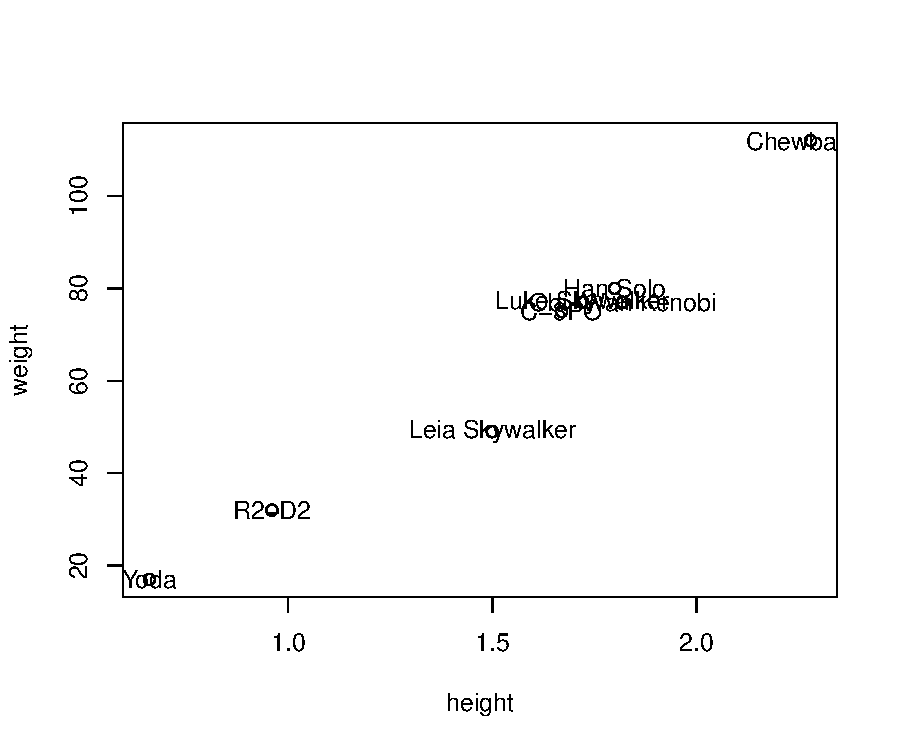
\includegraphics[width=.8\linewidth,height=.7\linewidth]{figure/sw_plot1-1} 

}



\end{knitrout}

\end{frame}

%------------------------------------------------

\begin{frame}[fragile]
\frametitle{Labeling Points with}

Use {\hilit \code{xpd = TRUE}} to expand the text outside the plotting region:
\begin{knitrout}\footnotesize
\definecolor{shadecolor}{rgb}{0.969, 0.969, 0.969}\color{fgcolor}\begin{kframe}
\begin{alltt}
\hlkwd{with}\hlstd{(sw,} \hlkwd{plot}\hlstd{(height, weight))}
\hlkwd{with}\hlstd{(sw,} \hlkwd{text}\hlstd{(height, weight,} \hlkwc{labels} \hlstd{= name,} \hlkwc{xpd} \hlstd{=} \hlnum{TRUE}\hlstd{))}
\end{alltt}
\end{kframe}
\end{knitrout}

\end{frame}

%------------------------------------------------

\begin{frame}[fragile]
\frametitle{Labeling Points with}

\begin{knitrout}\footnotesize
\definecolor{shadecolor}{rgb}{0.969, 0.969, 0.969}\color{fgcolor}

{\centering 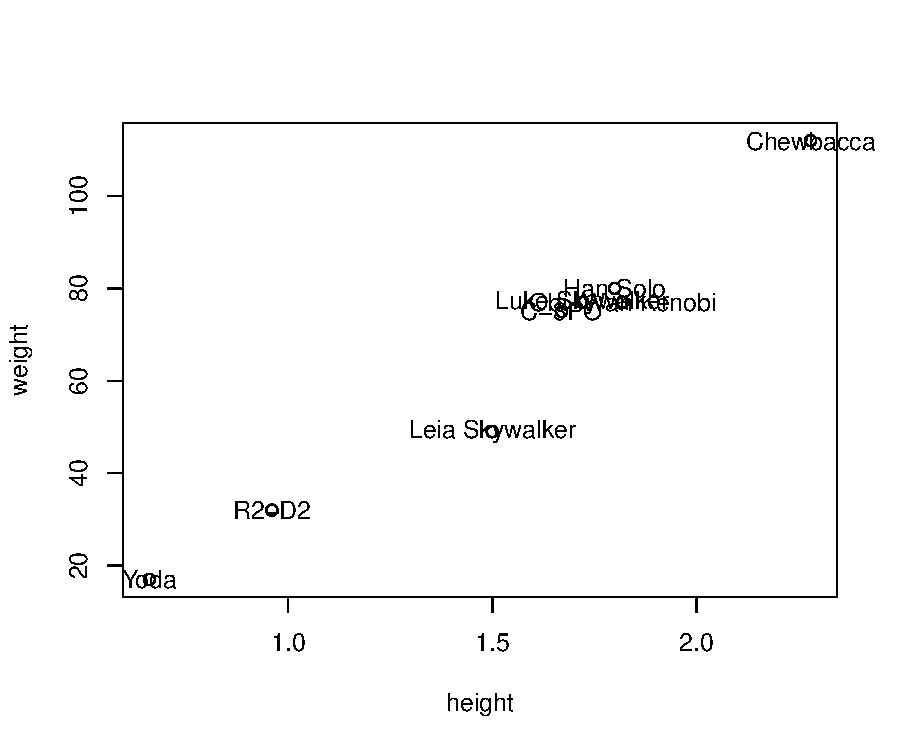
\includegraphics[width=.8\linewidth,height=.7\linewidth]{figure/sw_plot2-1} 

}



\end{knitrout}

{\footnotesize Some labels are not clearly displayed}
\end{frame}

%------------------------------------------------

\begin{frame}
\frametitle{Labeling Points}

\begin{center}
  \begin{tabular}{l l}
  \hline
  Acronym & Description \\
    \hline
    \code{text()} & Base R \\
    \code{spread.labels()} & \code{"plotrix"} \\
    \code{thigmophobe.labels()} & \code{"plotrix"} \\
    \code{pointLabel()} & \code{"maptools"} \\
\hline
 \end{tabular}
\end{center}


\end{frame}

%------------------------------------------------

\begin{frame}[fragile]
\frametitle{Labeling with \code{spread.labels()}}

Instead of \code{text()} we can use {\hilit \code{spread.labels()}}:
\begin{knitrout}\footnotesize
\definecolor{shadecolor}{rgb}{0.969, 0.969, 0.969}\color{fgcolor}\begin{kframe}
\begin{alltt}
\hlkwd{with}\hlstd{(sw,} \hlkwd{plot}\hlstd{(height, weight))}
\hlkwd{with}\hlstd{(sw,} \hlkwd{spread.labels}\hlstd{(height, weight,} \hlkwc{labels} \hlstd{= name))}
\end{alltt}
\end{kframe}
\end{knitrout}

\end{frame}

%------------------------------------------------

\begin{frame}[fragile]
\frametitle{Labeling with \code{spread.labels()}}

\begin{knitrout}\footnotesize
\definecolor{shadecolor}{rgb}{0.969, 0.969, 0.969}\color{fgcolor}

{\centering 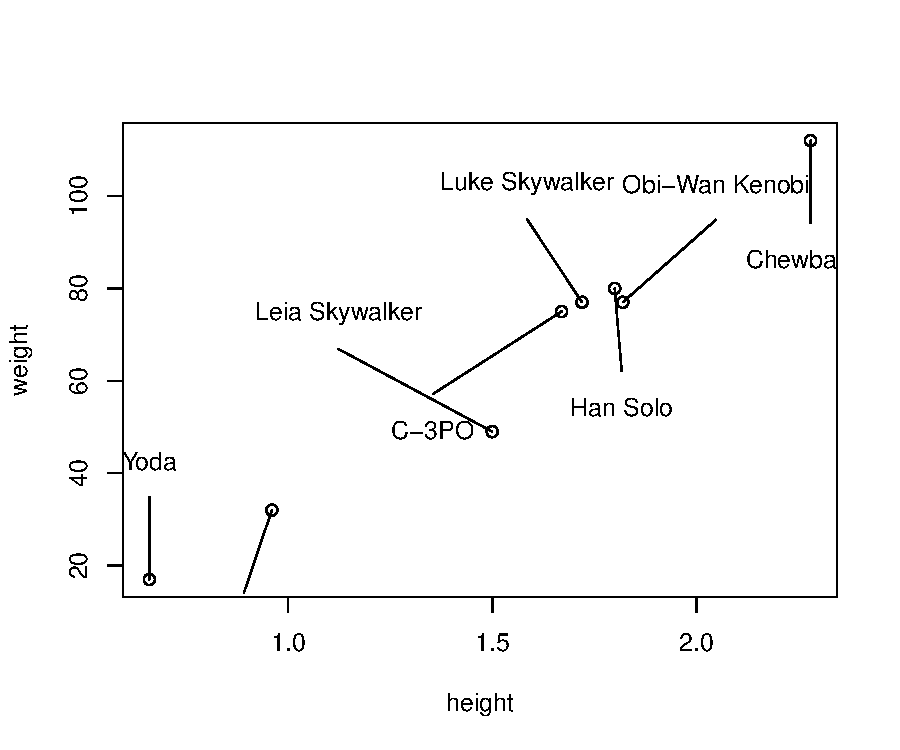
\includegraphics[width=.8\linewidth,height=.7\linewidth]{figure/sw_plot3-1} 

}



\end{knitrout}

\end{frame}

%------------------------------------------------

\begin{frame}[fragile]
\frametitle{Labeling with \code{thigmophobe.labels()}}

We can also use {\hilit \code{thigmophobe.labels()}}:
\begin{knitrout}\footnotesize
\definecolor{shadecolor}{rgb}{0.969, 0.969, 0.969}\color{fgcolor}\begin{kframe}
\begin{alltt}
\hlkwd{with}\hlstd{(sw,} \hlkwd{plot}\hlstd{(height, weight))}
\hlkwd{with}\hlstd{(sw,} \hlkwd{thigmophobe.labels}\hlstd{(height, weight,} \hlkwc{labels} \hlstd{= name))}
\end{alltt}
\end{kframe}
\end{knitrout}

\end{frame}

%------------------------------------------------

\begin{frame}[fragile]
\frametitle{Labeling with \code{spread.labels()}}

\begin{knitrout}\footnotesize
\definecolor{shadecolor}{rgb}{0.969, 0.969, 0.969}\color{fgcolor}

{\centering 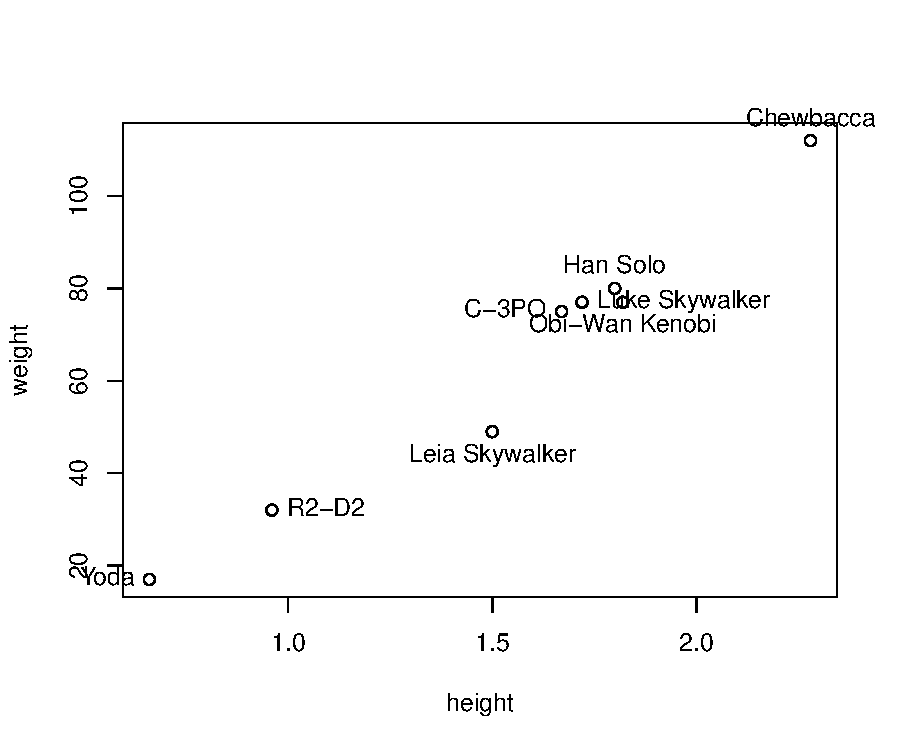
\includegraphics[width=.8\linewidth,height=.7\linewidth]{figure/sw_plot4-1} 

}



\end{knitrout}

\end{frame}

%------------------------------------------------

\begin{frame}[fragile]
\frametitle{Labeling with \code{pointLabel()}}

We can also use {\hilit \code{pointLabel()}}:
\begin{knitrout}\footnotesize
\definecolor{shadecolor}{rgb}{0.969, 0.969, 0.969}\color{fgcolor}\begin{kframe}
\begin{alltt}
\hlkwd{with}\hlstd{(sw,} \hlkwd{plot}\hlstd{(height, weight))}
\hlkwd{with}\hlstd{(sw,} \hlkwd{pointLabel}\hlstd{(height, weight,} \hlkwc{labels} \hlstd{= name))}
\end{alltt}
\end{kframe}
\end{knitrout}

\end{frame}

%------------------------------------------------

\begin{frame}[fragile]
\frametitle{Labeling with \code{pointLabel()}}

\begin{knitrout}\footnotesize
\definecolor{shadecolor}{rgb}{0.969, 0.969, 0.969}\color{fgcolor}

{\centering 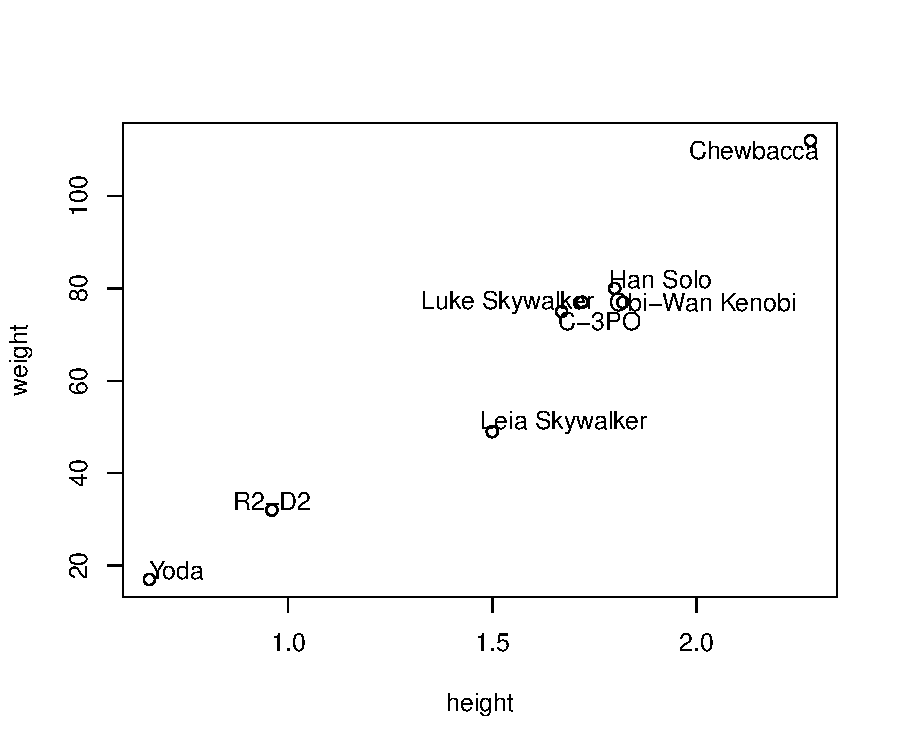
\includegraphics[width=.8\linewidth,height=.7\linewidth]{figure/sw_plot5-1} 

}



\end{knitrout}

\end{frame}

%------------------------------------------------

\begin{frame}
\begin{center}
\Huge{\hilit{Fonts \& Formulae}}
\end{center}
\end{frame}

%------------------------------------------------

\begin{frame}
\frametitle{Text and expressions}

\bi
  \item We can draw text with \code{text()}
  \item \code{text()} accepts character strings
  \item But it also accepts R expressions resulting from a call to {\hilit \code{expression()}}
  \item An expression is interpreted as a mathematical formula
  \item See \code{?plotmath} for more info
\ei

\end{frame}

%------------------------------------------------

\begin{frame}[fragile]
\frametitle{Text and expressions}

\begin{knitrout}\footnotesize
\definecolor{shadecolor}{rgb}{0.969, 0.969, 0.969}\color{fgcolor}\begin{kframe}
\begin{alltt}
\hlstd{op} \hlkwb{<-} \hlkwd{par}\hlstd{(}\hlkwc{mar} \hlstd{=} \hlkwd{c}\hlstd{(}\hlnum{4}\hlstd{,} \hlnum{4}\hlstd{,} \hlnum{1}\hlstd{,} \hlnum{1}\hlstd{))}
\hlkwd{plot.new}\hlstd{()}
\hlkwd{plot.window}\hlstd{(}\hlkwc{xlim} \hlstd{=} \hlkwd{c}\hlstd{(}\hlnum{0}\hlstd{,} \hlnum{1}\hlstd{),} \hlkwc{ylim} \hlstd{=} \hlkwd{c}\hlstd{(}\hlnum{0}\hlstd{,} \hlnum{1}\hlstd{))}
\hlkwd{axis}\hlstd{(}\hlkwc{side} \hlstd{=} \hlnum{1}\hlstd{)}
\hlkwd{axis}\hlstd{(}\hlkwc{side} \hlstd{=} \hlnum{2}\hlstd{)}
\hlkwd{text}\hlstd{(}\hlnum{0.5}\hlstd{,} \hlnum{0.8}\hlstd{,}
     \hlkwd{expression}\hlstd{(}\hlkwd{paste}\hlstd{(}\hlstr{"Temperature ("}\hlstd{, degree,} \hlstr{"C) in 2015"}\hlstd{)))}
\hlkwd{text}\hlstd{(}\hlnum{0.5}\hlstd{,} \hlnum{0.6}\hlstd{,}
     \hlkwd{expression}\hlstd{(}\hlkwd{bar}\hlstd{(x)} \hlopt{==} \hlkwd{sum}\hlstd{(}\hlkwd{frac}\hlstd{(x[i], n), i}\hlopt{==}\hlnum{1}\hlstd{, n)))}
\hlkwd{text}\hlstd{(}\hlnum{0.5}\hlstd{,} \hlnum{0.4}\hlstd{,}
     \hlkwd{expression}\hlstd{(}\hlkwd{hat}\hlstd{(beta)} \hlopt{==} \hlstd{(X}\hlopt{^}\hlstd{t} \hlopt{*} \hlstd{X)}\hlopt{^}\hlstd{(}\hlopt{-}\hlnum{1}\hlstd{)} \hlopt{*} \hlstd{X}\hlopt{^}\hlstd{t} \hlopt{*} \hlstd{y))}
\hlkwd{text}\hlstd{(}\hlnum{0.5}\hlstd{,} \hlnum{0.2}\hlstd{,}
     \hlkwd{expression}\hlstd{(z[i]} \hlopt{==} \hlkwd{sqrt}\hlstd{(x[i]}\hlopt{^}\hlnum{2} \hlopt{+} \hlstd{y[i]}\hlopt{^}\hlnum{2}\hlstd{)))}
\hlkwd{par}\hlstd{(op)}
\end{alltt}
\end{kframe}
\end{knitrout}

\end{frame}

%------------------------------------------------

\begin{frame}[fragile]
\frametitle{Text and expressions}

\begin{knitrout}\footnotesize
\definecolor{shadecolor}{rgb}{0.969, 0.969, 0.969}\color{fgcolor}

{\centering 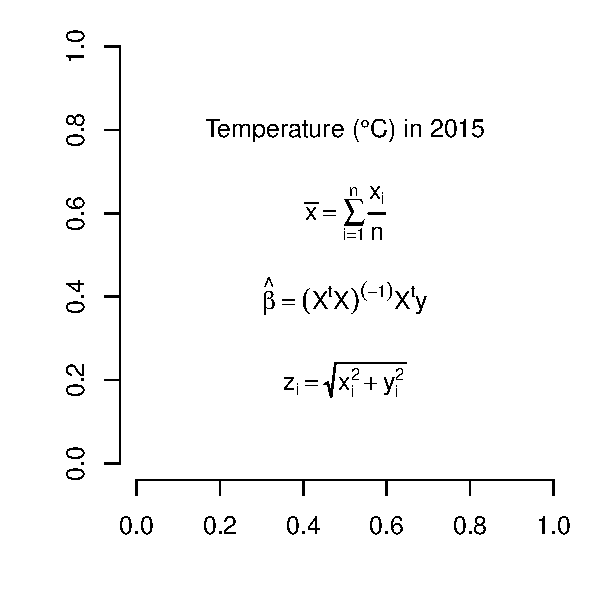
\includegraphics[width=.8\linewidth,height=.8\linewidth]{figure/formula-1} 

}



\end{knitrout}

\end{frame}

%------------------------------------------------

\begin{frame}
\frametitle{Text and expressions}

\bi
  \item We can draw text with \code{text()}
  \item \code{text()} accepts character strings
  \item But it also accepts R expressions resulting from a call to {\hilit \code{expression()}}
  \item An expressio nis interpreted as a mathematical formula
  \item See \code{?plotmath} for more info
\ei

\end{frame}

%------------------------------------------------

\begin{frame}[fragile]
\frametitle{Text and expressions}

How to pass a variable to an expression?
\begin{knitrout}\footnotesize
\definecolor{shadecolor}{rgb}{0.969, 0.969, 0.969}\color{fgcolor}\begin{kframe}
\begin{alltt}
\hlstd{year} \hlkwb{<-} \hlnum{2015}

\hlstd{op} \hlkwb{<-} \hlkwd{par}\hlstd{(}\hlkwc{mar} \hlstd{=} \hlkwd{c}\hlstd{(}\hlnum{4}\hlstd{,} \hlnum{4}\hlstd{,} \hlnum{1}\hlstd{,} \hlnum{1}\hlstd{))}
\hlkwd{plot.new}\hlstd{()}
\hlkwd{plot.window}\hlstd{(}\hlkwc{xlim} \hlstd{=} \hlkwd{c}\hlstd{(}\hlnum{0}\hlstd{,} \hlnum{1}\hlstd{),} \hlkwc{ylim} \hlstd{=} \hlkwd{c}\hlstd{(}\hlnum{0.4}\hlstd{,} \hlnum{0.6}\hlstd{))}
\hlkwd{axis}\hlstd{(}\hlkwc{side} \hlstd{=} \hlnum{1}\hlstd{)}
\hlkwd{axis}\hlstd{(}\hlkwc{side} \hlstd{=} \hlnum{2}\hlstd{)}
\hlkwd{text}\hlstd{(}\hlnum{0.5}\hlstd{,} \hlnum{0.5}\hlstd{,}
     \hlkwd{expression}\hlstd{(}\hlkwd{paste}\hlstd{(}\hlstr{"Temperature ("}\hlstd{, degree,} \hlstr{"C) in "}\hlstd{, year)))}
\hlkwd{par}\hlstd{(op)}
\end{alltt}
\end{kframe}
\end{knitrout}

\end{frame}

%------------------------------------------------

\begin{frame}[fragile]
\frametitle{Text and expressions}

\begin{knitrout}\footnotesize
\definecolor{shadecolor}{rgb}{0.969, 0.969, 0.969}\color{fgcolor}

{\centering 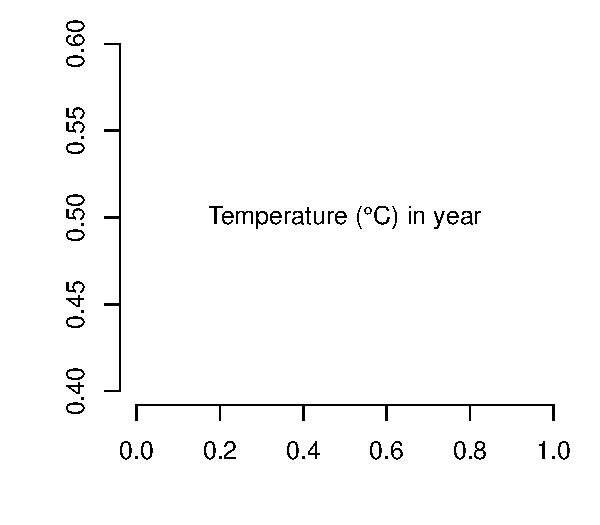
\includegraphics[width=.8\linewidth,height=.7\linewidth]{figure/formula2-1} 

}



\end{knitrout}

\end{frame}

%------------------------------------------------

\begin{frame}[fragile]
\frametitle{Text and expressions}

Passing a variable with {\hilit \code{substitute()}}
\begin{knitrout}\footnotesize
\definecolor{shadecolor}{rgb}{0.969, 0.969, 0.969}\color{fgcolor}\begin{kframe}
\begin{alltt}
\hlstd{year} \hlkwb{<-} \hlnum{2015}

\hlstd{op} \hlkwb{<-} \hlkwd{par}\hlstd{(}\hlkwc{mar} \hlstd{=} \hlkwd{c}\hlstd{(}\hlnum{4}\hlstd{,} \hlnum{4}\hlstd{,} \hlnum{1}\hlstd{,} \hlnum{1}\hlstd{))}
\hlkwd{plot.new}\hlstd{()}
\hlkwd{plot.window}\hlstd{(}\hlkwc{xlim} \hlstd{=} \hlkwd{c}\hlstd{(}\hlnum{0}\hlstd{,} \hlnum{1}\hlstd{),} \hlkwc{ylim} \hlstd{=} \hlkwd{c}\hlstd{(}\hlnum{0.4}\hlstd{,} \hlnum{0.6}\hlstd{))}
\hlkwd{axis}\hlstd{(}\hlkwc{side} \hlstd{=} \hlnum{1}\hlstd{)}
\hlkwd{axis}\hlstd{(}\hlkwc{side} \hlstd{=} \hlnum{2}\hlstd{)}
\hlkwd{text}\hlstd{(}\hlnum{0.5}\hlstd{,} \hlnum{0.5}\hlstd{,}
     \hlkwd{substitute}\hlstd{(}
       \hlkwd{paste}\hlstd{(}\hlstr{"Temperature ("}\hlstd{, degree,} \hlstr{"C) in "}\hlstd{, year),}
       \hlkwd{list}\hlstd{(}\hlkwc{year} \hlstd{= year))}
     \hlstd{)}
\hlkwd{par}\hlstd{(op)}
\end{alltt}
\end{kframe}
\end{knitrout}

\end{frame}

%------------------------------------------------

\begin{frame}[fragile]
\frametitle{Text and expressions}

\begin{knitrout}\footnotesize
\definecolor{shadecolor}{rgb}{0.969, 0.969, 0.969}\color{fgcolor}

{\centering 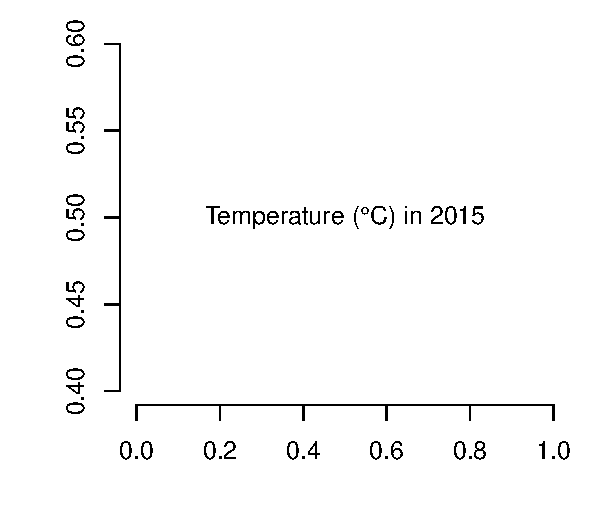
\includegraphics[width=.8\linewidth,height=.7\linewidth]{figure/formula3-1} 

}



\end{knitrout}

\end{frame}

%------------------------------------------------

\begin{frame}
\begin{center}
\Huge{\hilit{R package \code{"googleVis"}}}
\end{center}
\end{frame}

%------------------------------------------------

\begin{frame}
\frametitle{Some packages}

\bi
  \item \code{"googleVis"}
  \item \code{"rCharts"}
  \item \code{"rMaps"}
  \item \code{"rgl"}  
\ei

\end{frame}

%------------------------------------------------

\begin{frame}[fragile]
\frametitle{\code{"googleVis"}}

\begin{knitrout}\footnotesize
\definecolor{shadecolor}{rgb}{0.969, 0.969, 0.969}\color{fgcolor}\begin{kframe}
\begin{alltt}
\hlkwd{install.packages}\hlstd{(}\hlstr{"googleVis"}\hlstd{)}

\hlkwd{library}\hlstd{(googleVis)}

\hlkwd{data}\hlstd{(Fruits)}
\end{alltt}
\end{kframe}
\end{knitrout}

\end{frame}

%------------------------------------------------

\begin{frame}[fragile]
\frametitle{\code{"googleVis"}}

\begin{knitrout}\footnotesize
\definecolor{shadecolor}{rgb}{0.969, 0.969, 0.969}\color{fgcolor}\begin{kframe}
\begin{alltt}
\hlstd{M} \hlkwb{<-} \hlkwd{gvisMotionChart}\hlstd{(Fruits,} \hlkwc{idvar}\hlstd{=}\hlstr{"Fruit"}\hlstd{,} \hlkwc{timevar}\hlstd{=}\hlstr{"Year"}\hlstd{)}

\hlkwd{str}\hlstd{(M)}

\hlkwd{print}\hlstd{(M)}

\hlkwd{plot}\hlstd{(M)}
\end{alltt}
\end{kframe}
\end{knitrout}

\end{frame}

%------------------------------------------------


\end{document}
